\documentclass[conf]{new-aiaa}
%\documentclass[journal]{new-aiaa} for journal papers
\usepackage[utf8]{inputenc}

\usepackage{graphicx}
\usepackage{amsmath}
\usepackage{longtable,tabularx}
\hypersetup{hidelinks}
\setlength\LTleft{0pt} 
\setlength{\emergencystretch}{1em}

\title{Numerical Study of Heating During Hypersonic Descent Inspired by the X-43}

\author{Daniel Nunez, Winston Chong, Akon Qiu, and LiChen Liao}

\begin{document}

\maketitle

\begin{abstract}
This study examines aerodynamic heating during a simplified hypersonic descent
inspired by the NASA X-43. A five-state initial-value problem describes altitude,
speed, flight-path angle, stagnation-region temperature, and constant vehicle mass.
The model includes altitude-dependent atmospheric density and gravity, constant
lift and drag coefficients, convective heating, and radiative cooling.
The equations are integrated using a classical fourth-order Runge--Kutta method
implemented from scratch. Timestep refinement demonstrates convergence toward
fourth-order accuracy, while exact special-case solutions, independent derivative
benchmarks, and a mechanical energy identity check the implementation. The baseline temperature peaks at
$2632.82~\mathrm{K}$. Increasing initial speed from $1700$ to
$2500~\mathrm{m/s}$ raises peak temperature from $2373.43$ to
$2962.27~\mathrm{K}$, whereas increasing emissivity from $0.5$ to $1.0$
reduces it from $3006.14$ to $2528.01~\mathrm{K}$.
These predictions describe the assumed model over a $400~\mathrm{s}$
observation interval rather than a validated reconstruction of an X-43 flight.
\end{abstract}

\section{Nomenclature}

{\renewcommand\arraystretch{1.0}
\noindent\begin{longtable}{@{}l @{\quad=\quad} l@{}}
$A$ & reference area, $\mathrm{m^2}$ \\
$C_A$ & effective heat capacity per unit area, $\mathrm{J/(m^2\,K)}$ \\
$C_D$, $C_L$ & drag and lift coefficients \\
$c_p$ & specific heat capacity, $\mathrm{J/(kg\,K)}$ \\
$D$, $L$ & drag and lift forces, $\mathrm{N}$ \\
$E$ & specific mechanical energy, $\mathrm{J/kg}$ \\
$g$, $g_0$ & local and surface gravitational accelerations, $\mathrm{m/s^2}$ \\
$H$ & atmospheric scale height, $\mathrm{m}$ \\
$h$, $h_0$ & altitude and baseline initial altitude, $\mathrm{m}$ \\
$K$ & convective-heating coefficient, $\mathrm{kg^{1/2}/m}$ \\
$m$ & vehicle mass, $\mathrm{kg}$ \\
$R_E$ & Earth radius, $\mathrm{m}$ \\
$R_n$ & nose radius, $\mathrm{m}$ \\
$T_s$ & approximate stagnation-region temperature, $\mathrm{K}$ \\
$V$ & vehicle speed, $\mathrm{m/s}$ \\
$\gamma$ & flight-path angle, $\mathrm{rad}$ \\
$\delta$ & effective heated thickness, $\mathrm{m}$ \\
$\epsilon$ & surface emissivity \\
$\rho_a$, $\rho_{30}$ & local and reference atmospheric densities, $\mathrm{kg/m^3}$ \\
$\rho_s$ & material density, $\mathrm{kg/m^3}$ \\
$\sigma$ & Stefan--Boltzmann constant, $\mathrm{W/(m^2\,K^4)}$ \\
$\dot q_{\mathrm{conv}}$ & convective heat flux, $\mathrm{W/m^2}$ \\
$Q_{\mathrm{conv}}$ & integrated convective heat load per unit area, $\mathrm{J/m^2}$ \\
$\Delta t$ & numerical timestep, $\mathrm{s}$
\end{longtable}}

\section{Introduction}

Hypersonic vehicles experience substantial aerodynamic heating, and their
thermal response depends on both the trajectory and the balance between
convective heating and radiative cooling. Inspired by the NASA X-43 program~\cite{nasa-x43}, this
study considers an unpowered vehicle beginning at $30~\mathrm{km}$ with
speed $2112.14~\mathrm{m/s}$, approximately Mach 7 under the assumed initial
conditions, flight-path angle $-2^\circ$, and mass $1400~\mathrm{kg}$.
The vehicle and material parameters are modeling assumptions rather than
verified X-43 flight data.

The primary questions are how initial speed affects convective heating and
peak temperature, and how emissivity affects the thermal response. A
supplementary study varies the initial flight-path angle. Addressing these
questions requires tracking how altitude-dependent density changes aerodynamic
forces and heating while the vehicle speed and trajectory evolve. These
nonlinear relationships, together with fourth-power radiative cooling,
produce a coupled initial-value problem without a known closed-form solution
for the full model. We therefore use numerical integration and assess its
accuracy through timestep refinement and independent implementation checks.

\section{Mathematical Model}

The vehicle is represented by a point mass with locally flat flight geometry.
Earth rotation and trajectory-curvature terms are neglected, while gravity
is allowed to vary with altitude. The state and initial-value problem are
\begin{equation}
\mathbf y=[h,\;V,\;\gamma,\;T_s,\;m]^T,
\qquad
\frac{d\mathbf y}{dt}=\mathbf f(t,\mathbf y),
\qquad
\mathbf y(0)=\mathbf y_0,
\end{equation}
with baseline initial conditions
\begin{equation}
\mathbf y_0=[30000,\;2112.14,\;-2\pi/180,\;300,\;1400]^T.
\end{equation}
The components use meters, meters per second, radians, kelvin, and kilograms,
respectively. A negative flight-path angle denotes descent.

\subsection{Flight Dynamics}

The translational equations are
\begin{align}
\frac{dh}{dt} &= V\sin\gamma, \\
\frac{dV}{dt} &= -\frac{D}{m}-g(h)\sin\gamma, \\
\frac{d\gamma}{dt} &= \frac{L}{mV}-\frac{g(h)\cos\gamma}{V}, \\
\frac{dm}{dt} &= 0.
\end{align}
Drag opposes motion, while lift and gravity change the flight-path angle.
Ablation is neglected, so mass remains constant.

The aerodynamic forces are
\begin{equation}
D=\frac12\rho_a(h)V^2C_DA,
\qquad
L=\frac12\rho_a(h)V^2C_LA.
\end{equation}
The coefficients $C_D$ and $C_L$ are constant; Mach-number and
angle-of-attack dependence are neglected. The forces still vary through
their dependence on speed and atmospheric density.

Density and gravitational acceleration are modeled as
\begin{equation}
\rho_a(h)=\rho_{30}\exp\left[-\frac{h-h_0}{H}\right],
\qquad
g(h)=g_0\left(\frac{R_E}{R_E+h}\right)^2,
\end{equation}
where $h_0=30000~\mathrm{m}$ is the fixed reference altitude.
The exponential density approximation couples altitude to aerodynamic forces
and heating.

\subsection{Thermal Response}

Convective heating is represented by a Sutton--Graves-type correlation~\cite{sutton-graves},
\begin{equation}
\dot q_{\mathrm{conv}}=K\sqrt{\frac{\rho_a(h)}{R_n}}V^3.
\end{equation}
This correlation estimates stagnation-point heating. Accordingly, $T_s$
represents an approximate stagnation-region temperature rather than a
uniform temperature over the aircraft.

An energy balance gives
\begin{equation}
\frac{dT_s}{dt}
=\frac{\dot q_{\mathrm{conv}}-\epsilon\sigma T_s^4}{C_A},
\qquad
C_A=\rho_s c_p\delta=7200~\mathrm{J/(m^2\,K)}.
\end{equation}
Incoming environmental radiation, conduction into the vehicle interior,
and material degradation are neglected. The effective carbon--carbon
material properties are assumed constant. Temperature does not feed back
into the aerodynamic forces or convective heating in this model.

\subsection{Baseline Parameter Values}

Table~\ref{tab:baseline-parameters} specifies the baseline parameters.
Vehicle geometry, aerodynamic coefficients, and material properties are
assumed inputs rather than verified X-43 measurements. Each parameter is
held constant within a run; only the selected study parameter changes
between runs.

\begin{table}[htbp]
\caption{Baseline model parameters.}
\label{tab:baseline-parameters}
\centering
\begin{tabular}{lll}
\hline
Parameter & Value & Units \\
\hline
Drag coefficient, $C_D$ & 0.02 & Dimensionless \\
Lift coefficient, $C_L$ & 0.080 & Dimensionless \\
Reference area, $A$ & 4.00 & $\mathrm{m^2}$ \\
Nose radius, $R_n$ & 0.010 & $\mathrm{m}$ \\
Surface emissivity, $\epsilon$ & 0.85 & Dimensionless \\
Specific heat, $c_p$ & 900 & $\mathrm{J/(kg\,K)}$ \\
Material density, $\rho_s$ & 1600 & $\mathrm{kg/m^3}$ \\
Heated thickness, $\delta$ & 0.005 & $\mathrm{m}$ \\
Reference air density, $\rho_{30}$ & 0.0184 & $\mathrm{kg/m^3}$ \\
Atmospheric scale height, $H$ & 7000 & $\mathrm{m}$ \\
Surface gravity, $g_0$ & 9.81 & $\mathrm{m/s^2}$ \\
Earth radius, $R_E$ & $6.371\times10^6$ & $\mathrm{m}$ \\
Heating coefficient, $K$ & $1.7415\times10^{-4}$ & $\mathrm{kg^{1/2}/m}$ \\
Stefan--Boltzmann constant, $\sigma$ & $5.670374419\times10^{-8}$ & $\mathrm{W/(m^2\,K^4)}$ \\
\hline
\end{tabular}
\end{table}

\section{Numerical Method}

\subsection{Selection of RK4}

The five-state IVP is integrated using the classical four-stage Runge--Kutta
method presented in Lecture 10~\cite{lecture10}, implemented from scratch. RK4 is explicit and requires four evaluations
of the complete derivative function per timestep, without a nonlinear algebraic
solve. For this small system, that cost makes repeated parameter studies
practical. Its fourth-order accuracy also reduces the number of steps needed
relative to a first-order method when both operate in their convergence regimes.
Timestep refinement is used to assess accuracy for the simulated conditions.

\subsection{RK4 Update}

Starting from time $t_k$ and state $\mathbf y_k$, the exact update satisfies
\begin{equation}
\mathbf y(t_k+\Delta t)
=\mathbf y(t_k)+\int_{t_k}^{t_k+\Delta t}\mathbf f(t,\mathbf y(t))\,dt.
\end{equation}
RK4 approximates this integral using four derivative estimates:
\begin{align}
\mathbf k_1 &= \mathbf f(t_k,\mathbf y_k), \\
\mathbf k_2 &= \mathbf f\left(t_k+\frac{\Delta t}{2},
                    \mathbf y_k+\frac{\Delta t}{2}\mathbf k_1\right), \\
\mathbf k_3 &= \mathbf f\left(t_k+\frac{\Delta t}{2},
                    \mathbf y_k+\frac{\Delta t}{2}\mathbf k_2\right), \\
\mathbf k_4 &= \mathbf f(t_k+\Delta t,\mathbf y_k+\Delta t\mathbf k_3).
\end{align}
The state is advanced by
\begin{equation}
\mathbf y_{k+1}=\mathbf y_k+
\frac{\Delta t}{6}(\mathbf k_1+2\mathbf k_2+2\mathbf k_3+\mathbf k_4).
\end{equation}
Each stage is a five-component vector. Density, gravity, aerodynamic forces,
and heat fluxes are recalculated at that stage's intermediate state, so the
entire coupled system is advanced together.


\subsection{Accuracy and Truncation Error}

Lecture 10 presents classical RK4 as a fourth-order one-step method~\cite{lecture10}.
Following Lecture 11, we examine accuracy by substituting the exact solution
into the update and comparing Taylor expansions~\cite{lecture11}.
For a smooth exact solution and $s=\Delta t$,
\begin{equation}
\mathbf y(t_k+s)=\mathbf y(t_k)
+s\mathbf y'(t_k)+\frac{s^2}{2}\mathbf y''(t_k)
+\frac{s^3}{6}\mathbf y^{(3)}(t_k)
+\frac{s^4}{24}\mathbf y^{(4)}(t_k)+\mathcal O(s^5).
\end{equation}
RK4 uses its two midpoint estimates and endpoint estimate to match these
terms through fourth order. The matching can be shown directly for the
scalar test equation $u'=\lambda u$. Starting from the exact value $u(t_k)$,
the four stages are
\begin{align}
k_1 &= \lambda u(t_k),\\
k_2 &= \lambda u(t_k)\left(1+\frac{\lambda s}{2}\right),\\
k_3 &= \lambda u(t_k)\left(1+\frac{\lambda s}{2}
                             +\frac{\lambda^2s^2}{4}\right),\\
k_4 &= \lambda u(t_k)\left(1+\lambda s+
                   \frac{\lambda^2s^2}{2}+\frac{\lambda^3s^3}{4}\right).
\end{align}
Substituting these expressions into the RK4 update gives
\begin{equation}
u_{k+1}=u(t_k)\left[1+\lambda s+\frac{\lambda^2s^2}{2}
 +\frac{\lambda^3s^3}{6}+\frac{\lambda^4s^4}{24}\right].
\end{equation}
The exact solution advances by $u(t_k+s)=u(t_k)e^{\lambda s}$, whose
Taylor series has the same terms through $s^4$. The difference after
one step is therefore $\mathcal O(s^5)$.

Using Lecture 11's convention, the truncation error is this one-step
residual divided by the timestep:
\begin{equation}
\tau_k=\frac{u(t_k+s)-u_{k+1}}{s}=\mathcal O(s^4).
\end{equation}
Thus the $\mathcal O(s^5)$ one-step solution error and the
$\mathcal O(s^4)$ truncation error describe the same calculation using
different conventions. For smooth problems with stable time integration,
RK4 has global error $\mathcal O(s^4)$ over a fixed interval. Halving
the timestep should therefore reduce that error by approximately sixteen.

The scalar calculation illustrates the Taylor matching; it is not a
proof of order for every nonlinear vector system. For the present coupled
model, the timestep study tests the expected fourth-order behavior directly,
and the exact drag and cooling cases independently check the computed solutions.

\subsection{Linear Stability}


Following Lecture 12, apply the numerical method to $u'=\lambda u$
and write the update as $u_{n+1}=R(w)u_n$, where
$w=\lambda\Delta t$~\cite{lecture12}. The stage substitution above gives
\begin{equation}
R(w)=1+w+\frac{w^2}{2}+\frac{w^3}{6}+\frac{w^4}{24}.
\end{equation}
For a decaying mode, $|R(w)|<1$ means that its numerical amplitude decreases;
$|R(w)|>1$ means it grows. The boundary is $|R(w)|=1$.
On the negative real axis, RK4 is stable for
$-2.78529<w<0$, consistent with the limit reported in Lecture 12.

Following the local linearization approach in Lectures 12--13~\cite{lecture12,lecture13},
the temperature derivative gives the thermal eigenvalue
\begin{equation}
\lambda_T=-\frac{4\epsilon\sigma T_s^3}{C_A}.
\end{equation}
Along the baseline trajectory, this gives a minimum
local thermal stability limit of approximately
$5.70~\mathrm{s}$. The selected timestep of
$0.1~\mathrm{s}$ is below this limit.
This calculation assesses the thermal mode only;
it does not establish stability of the complete
nonlinear system. Full-model convergence and
parameter-case refinement provide additional
numerical evidence. At the production step, the baseline takes $4000$ ordinary
steps and $16000$ RK4 stage evaluations. This cost is modest for five states,
and no implicit equation solves are needed.

\subsection{Algorithmic Implementation}

At each step, the code evaluates the four stage vectors, forms the weighted
update, stores the new state, and advances time. The last step is shortened
when necessary to end at the requested final time. If a step crosses the
specified altitude threshold, the code locates the crossing by repeatedly
halving the bracketed time interval and recomputing a shortened RK4 step.
This stopping calculation is not used in any reported case because all
cases reach the time horizon first. Integration stops at that
event or at the time horizon, whichever occurs first.

\section{Implementation Verification and Timestep Selection}

\subsection{Timestep-Convergence Study}

The baseline five-state IVP was integrated over
$0 \leq t \leq 400~\mathrm{s}$ using timesteps of
$1.0$, $0.5$, $0.25$, and $0.125~\mathrm{s}$.
The initial conditions and physical parameters were held fixed.
A reference solution was computed using the same from-scratch
RK4 implementation with
$\Delta t_{\mathrm{ref}}=0.03125~\mathrm{s}$.
All comparisons were made at matching time nodes, so interpolation
was unnecessary.

For each state component $j$, the maximum error relative to the
reference was defined as
\begin{equation}
E_j(\Delta t)
=
\max_n
\left|
y_j^{(\Delta t)}(t_n)
-
y_j^{(\mathrm{ref})}(t_n)
\right|.
\end{equation}
The observed convergence order was calculated from successive
timestep refinements:
\begin{equation}
p_j
=
\log_2
\left(
\frac{E_j(\Delta t)}
     {E_j(\Delta t/2)}
\right).
\end{equation}
For a fourth-order method, $p_j$ should approach four, corresponding
to an error reduction of approximately sixteen when the timestep
is halved.

\begin{table}[htbp]
\caption{Full-IVP convergence against an RK4 reference with
$\Delta t_{\mathrm{ref}}=0.03125~\mathrm{s}$. The order in each
row compares that row with the preceding row.}
\label{tab:flight-convergence}
\centering
\small
\begin{tabular}{ccccc}
\hline
$\Delta t$ (s) &
$E_h$ (m) &
$E_V$ (m/s) &
$E_{T_s}$ (K) &
$p_{T_s}$ \\
\hline
1.000 & $1.72162\times10^{-4}$ &
$2.23630\times10^{-6}$ &
$5.91707\times10^{-2}$ & --- \\
0.500 & $1.07599\times10^{-5}$ &
$1.39611\times10^{-7}$ &
$3.22222\times10^{-3}$ & 4.199 \\
0.250 & $6.72269\times10^{-7}$ &
$8.71842\times10^{-9}$ &
$1.88395\times10^{-4}$ & 4.096 \\
0.125 & $4.18695\times10^{-8}$ &
$5.52291\times10^{-10}$ &
$1.13451\times10^{-5}$ & 4.054 \\
\hline
\end{tabular}
\end{table}

Table~\ref{tab:flight-convergence} shows that the observed
temperature order approaches four as the timestep decreases.
Altitude and velocity errors also decrease by approximately
a factor of sixteen with each refinement.
These results demonstrate the expected fourth-order behavior
for the coupled flight and thermal calculation.

Because the reference solution is numerical, this study establishes
self-convergence rather than an independent verification of the
governing equations. The exact special-case solutions, derivative benchmarks, and mechanical energy check below
address that separate requirement.

\subsection{Independent Verification Against Exact Special Cases}

Self-convergence cannot show that the correct equations have been solved.
Two analytically solvable limits were therefore integrated using the same
five-state model function and RK4 routine as the full problem. Only parameters
and initial conditions were changed; no separate simplified numerical
right-hand side was used.

\subsubsection{Constant-altitude drag}

Set $g_0=0$, $C_L=0$, and $\gamma_0=0$, and disable convective heating and
radiation. Then $h$, $\gamma$, $T_s$, and $m$ remain constant, and density is
fixed at $\rho_a(h_0)$. The velocity equation reduces to
\begin{equation}
\frac{dV}{dt}=-aV^2,
\qquad a=\frac{\rho_a(h_0)C_D A}{2m_0}.
\end{equation}
Integrating $dV/V^2=-a\,dt$ gives
\begin{equation}
V_{\mathrm{exact}}(t)=\frac{V_0}{1+aV_0t}.
\end{equation}
This test uses $h_0=30000~\mathrm{m}$, $V_0=2112.14~\mathrm{m/s}$,
$T_{s,0}=300~\mathrm{K}$, $m_0=1400~\mathrm{kg}$, and a $20~\mathrm{s}$
interval. For this verification experiment only, $C_D=2$ makes the
truncation error measurable above floating-point roundoff. Production
simulations retain $C_D=0.02$.

\begin{table}[htbp]
\caption{Convergence to the exact constant-altitude drag solution.
Error is the maximum speed difference at sampled time nodes.}
\label{tab:exact-drag}
\centering
\begin{tabular}{ccc}
\hline
$\Delta t$ (s) & Maximum error (m/s) & Observed order\\
\hline
2.000 & $1.97324\times10^{-2}$ & ---\\
1.000 & $1.40536\times10^{-3}$ & 3.812\\
0.500 & $8.99864\times10^{-5}$ & 3.965\\
0.250 & $5.66429\times10^{-6}$ & 3.990\\
0.125 & $3.54472\times10^{-7}$ & 3.998\\
\hline
\end{tabular}
\end{table}
Table~\ref{tab:exact-drag} shows convergence to an independently known
solution, with order approaching four. This checks the drag sign,
coefficient and mass dependence, and its time integration in this limit.

\subsubsection{Radiative cooling}

Set atmospheric density and gravity to zero and choose $\gamma_0=0$.
The flight variables remain constant, convective heating vanishes, and
\begin{equation}
\frac{dT_s}{dt}=-\frac{\epsilon\sigma}{C_A}T_s^4.
\end{equation}
Integrating $T_s^{-4}dT_s=-(\epsilon\sigma/C_A)dt$ yields
\begin{equation}
T_{s,\mathrm{exact}}(t)=
\left(T_{s,0}^{-3}+\frac{3\epsilon\sigma}{C_A}t\right)^{-1/3}.
\end{equation}
Using $T_{s,0}=2500~\mathrm{K}$, $\epsilon=0.85$, and
$C_A=7200~\mathrm{J/(m^2\,K)}$ over $20~\mathrm{s}$ gives
Table~\ref{tab:exact-cooling}. Other initial flight variables retain their
baseline values except for $\gamma_0=0$.

\begin{table}[htbp]
\caption{Convergence to the exact radiative-cooling solution.
Errors are maximum temperature differences at sampled time nodes.}
\label{tab:exact-cooling}
\centering
\begin{tabular}{ccc}
\hline
$\Delta t$ (s) & Maximum error (K) & Observed order\\
\hline
0.25000 & $7.19051\times10^{-6}$ & ---\\
0.12500 & $2.87742\times10^{-7}$ & 4.643\\
0.06250 & $1.32186\times10^{-8}$ & 4.444\\
0.03125 & $6.81212\times10^{-10}$ & 4.278\\
\hline
\end{tabular}
\end{table}
The errors decrease toward the exact cooling solution, checking the radiation
sign, fourth-power temperature dependence, and heat-capacity factor. The
apparent orders above four at these steps approach four under refinement;
they do not imply a higher formal order for RK4.

\begin{figure}[htbp]
\centering
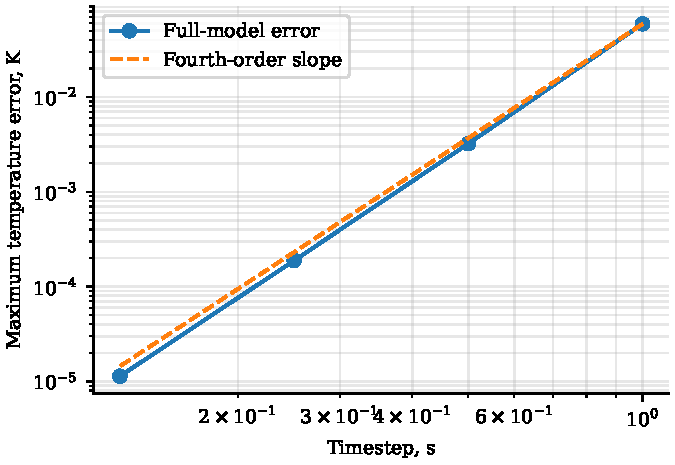
\includegraphics[width=0.72\linewidth]{figures/flight_convergence.pdf}
\caption{Full-model maximum temperature error under timestep refinement,
compared with a fourth-order slope. Independent exact-solution results
are reported in Tables~\ref{tab:exact-drag} and~\ref{tab:exact-cooling}.}
\label{fig:convergence}
\end{figure}

\subsection{Derivative Benchmarks and Mechanical Energy Check}

To complement the exact limits, the complete derivative function was
checked against independent calculations at two prescribed operating states.

Two prescribed states were selected:
\begin{align}
\mathbf{y}_A &=
[30000,\;2112.14,\;-2\pi/180,\;300,\;1400]^T,\\
\mathbf{y}_B &=
[20000,\;1800,\;-4\pi/180,\;2200,\;1400]^T.
\end{align}
The state components use meters, meters per second, radians,
kelvin, and kilograms, respectively. State A represents the
baseline initial condition. State B checks the equations at
a lower altitude and higher surface temperature, where
atmospheric density and radiative cooling differ substantially.

For each state, density and gravity were evaluated independently.
Drag, lift, and both heat fluxes were then calculated using scalar
arithmetic without the project's model helper functions. Substitution
into the five governing equations gave the benchmark derivatives.

\begin{table}[htbp]
\caption{Independent derivative benchmarks. Values shown
are rounded for presentation.}
\label{tab:derivative-verification}
\centering
\begin{tabular}{lcc}
\hline
Derivative & State A & State B \\
\hline
$\dot h$ (m/s) &
$-73.71262297$ & $-125.56165274$ \\
$\dot V$ (m/s$^2$) &
$-2.00612018$ & $-6.42744249$ \\
$\dot\gamma$ (rad/s) &
$-1.56812807\times10^{-4}$ &
$1.03916439\times10^{-2}$ \\
$\dot T_s$ (K/s) &
$309.09488520$ & $234.05040846$ \\
$\dot m$ (kg/s) & $0$ & $0$ \\
\hline
\end{tabular}
\end{table}

The implemented derivative function matched the unrounded
benchmark values using relative and absolute tolerances
of $10^{-12}$. This comparison checks the signs, coefficients,
and state dependence of the implemented equations at two
distinct operating conditions.

An additional check used an independently derived mechanical
energy identity. Define the specific mechanical energy as
\begin{equation}
E =
\frac{V^2}{2}
+
\frac{g_0 R_E h}{R_E+h}.
\end{equation}
The derivative of the potential-energy term with respect to
altitude is $g(h)$. Therefore,
\begin{equation}
\frac{dE}{dt}
=
V\frac{dV}{dt}
+
g(h)\frac{dh}{dt}.
\end{equation}
Substituting the governing equations gives
\begin{equation}
\frac{dE}{dt}
=
V\left(-\frac{D}{m}-g\sin\gamma\right)
+
gV\sin\gamma
=
-\frac{DV}{m}.
\end{equation}
Thus, gravity transfers energy between kinetic and potential
forms, while drag removes mechanical energy. The implemented
derivatives satisfied this identity at the baseline initial
state to a relative tolerance of $10^{-13}$.

Together, the exact special cases, independent derivative benchmarks, and mechanical
energy check provide evidence that the governing equations
were translated into code correctly. The timestep-convergence
study separately demonstrates the expected fourth-order
behavior of RK4. These checks verify numerical implementation;
they do not validate the physical assumptions of the model.
\subsection{Selection of the Production Timestep}

A production timestep of $0.1~\mathrm{s}$ was selected.
Each of the 22 parameter cases was repeated using
$0.05~\mathrm{s}$. The acceptance criteria were a
peak-temperature change below $0.5~\mathrm{K}$ and
relative changes below $0.1\%$ in both peak convective
heat flux and integrated convective heat load.

All cases satisfied these criteria. The largest change
in peak temperature was $6.53429\times10^{-4}~\mathrm{K}$.
Together with the convergence study, these results
support the selected timestep for the reported studies. The largest relative
changes in peak flux and integrated heat load are approximately
$4.84\times10^{-7}$ and $4.40\times10^{-8}$, respectively. These differences
are empirical accuracy indicators rather than rigorous error bounds. Peak
differences include sampling effects; heat load additionally has trapezoidal
quadrature error.

\section{Results}

Each simulation ends at $400~\mathrm{s}$ or the first downward crossing of
$10~\mathrm{km}$. All reported cases reached the time horizon first, so the
results describe a common observation interval rather than a complete descent.
The parameter studies vary one quantity at a time: initial speed from
$1700$ to $2500~\mathrm{m/s}$ in $100~\mathrm{m/s}$ increments,
initial flight-path angle from $-6^\circ$ to $0^\circ$ in $1^\circ$ increments,
and emissivity from $0.5$ to $1.0$ in increments of $0.1$.
Other inputs retain their baseline values.

In addition to peak temperature and peak flux, the integrated convective
heat load per unit area is
\begin{equation}
Q_{\mathrm{conv}}=\int_0^{t_{\mathrm{end}}}\dot q_{\mathrm{conv}}(t)\,dt,
\end{equation}
evaluated using the composite trapezoidal rule. Reported peaks are maxima
sampled at the numerical time nodes; the step-halving study checks the
sensitivity of these quantities to temporal resolution.

\subsection{Baseline Simulation}

Using the baseline state and parameters with $\Delta t=0.1~\mathrm{s}$,
the temperature reaches $2632.82~\mathrm{K}$ at approximately
$28~\mathrm{s}$. Peak convective heat flux is $2.317~\mathrm{MW/m^2}$,
and integrated convective heat load is $563.57~\mathrm{MJ/m^2}$.
At $400~\mathrm{s}$, altitude is $21.34~\mathrm{km}$ and speed is
$1178.83~\mathrm{m/s}$.

Figure~\ref{fig:baseline} shows the trajectory and thermal histories.
The altitude oscillations arise because lift changes the flight-path angle.
During descent, increasing density can raise lift above $mg\cos\gamma$,
turning the trajectory upward. As the vehicle climbs, density and lift decrease,
allowing gravity to turn the trajectory downward again. Drag removes mechanical
energy throughout, producing an overall descent with temporary climbs.
This behavior is a prediction of the simplified equations rather than a
validated X-43 flight characteristic.

\begin{figure}[t]
\centering
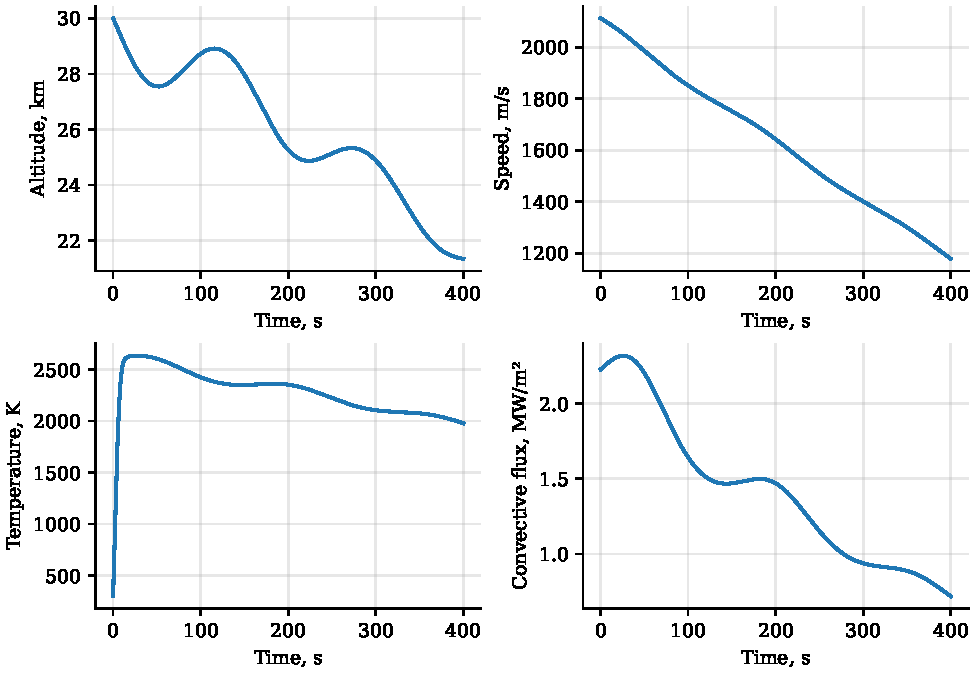
\includegraphics[width=\linewidth]{figures/baseline.pdf}
\caption{Baseline altitude, speed, approximate stagnation-region temperature,
and convective heat flux over the $400~\mathrm{s}$ observation interval.}
\label{fig:baseline}
\end{figure}

\subsection{Effect of Initial Velocity}

As shown in Fig.~\ref{fig:velocity-study}, increasing initial speed from
$1700$ to $2500~\mathrm{m/s}$ increases peak convective heat flux from
$1.532$ to $3.732~\mathrm{MW/m^2}$ and peak temperature from
$2373.43$ to $2962.27~\mathrm{K}$. This trend is consistent with the
$V^3$ dependence of convective heating. The peak values also depend on
how the changed initial speed modifies the subsequent density and trajectory
histories, so they cannot be inferred from the initial-speed ratio alone.
Integrated heat load also increases from $335.56$ to
$837.50~\mathrm{MJ/m^2}$ over the observation interval. Thus both the
instantaneous heating demand and cumulative exposure increase with initial
speed over this range.


\begin{figure}[htbp]
\centering
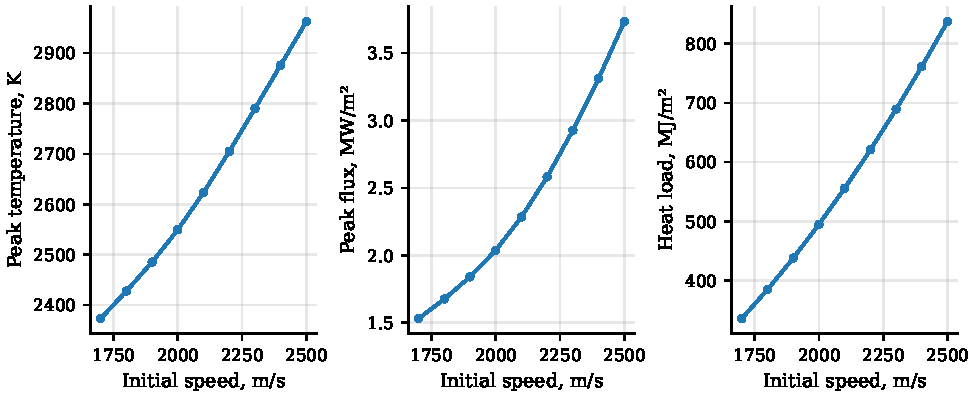
\includegraphics[width=\linewidth]{figures/velocity_study.pdf}
\caption{Effect of initial speed on peak temperature, peak convective flux,
and integrated heat load. Other inputs retain baseline values.}
\label{fig:velocity-study}
\end{figure}

\subsection{Effect of Surface Emissivity}

Figure~\ref{fig:emissivity-study} shows that increasing emissivity from
$0.5$ to $1.0$ reduces peak temperature from
$3006.14$ to $2528.01~\mathrm{K}$, while peak convective heat flux remains
$2.317~\mathrm{MW/m^2}$. Higher emissivity increases radiative heat loss.
Because temperature does not feed back into the flight equations, the
trajectory and incoming convective heat flux are unchanged in this study.
The integrated incoming heat load remains $563.57~\mathrm{MJ/m^2}$.
Emissivity controls outgoing radiation while leaving incoming heating unchanged.


\begin{figure}[htbp]
\centering
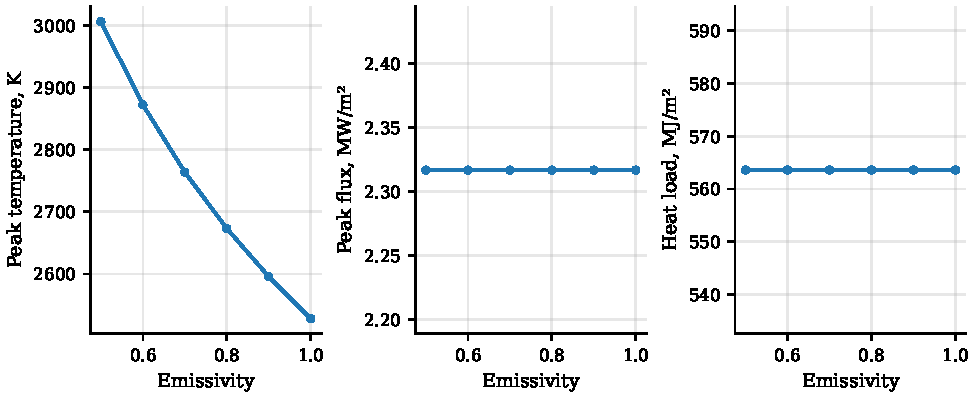
\includegraphics[width=\linewidth]{figures/emissivity_study.pdf}
\caption{Effect of emissivity on peak temperature, peak convective flux,
and integrated heat load. The trajectory and incoming heating are unchanged.}
\label{fig:emissivity-study}
\end{figure}

\subsection{Effect of Initial Flight-Path Angle}

The supplementary angle study in Fig.~\ref{fig:angle-study} shows that
changing the initial angle from $0^\circ$ to $-6^\circ$ raises peak
temperature from $2572.17$ to $2777.78~\mathrm{K}$ and peak convective
heat flux from $2.226$ to $2.873~\mathrm{MW/m^2}$. However, integrated
heat load decreases from $566.00$ to $549.11~\mathrm{MJ/m^2}$ over the
fixed observation interval. Peak heating and cumulative exposure therefore
need not change in the same direction when the trajectory changes.

\begin{figure}[t]
\centering
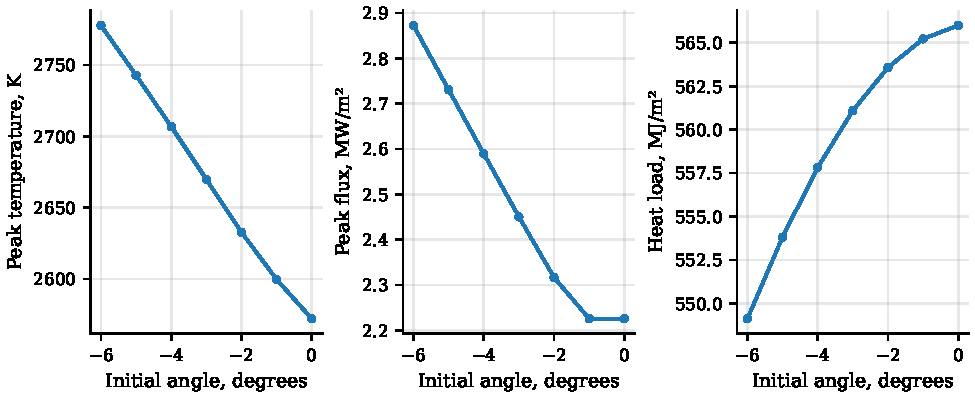
\includegraphics[width=\linewidth]{figures/angle_study.pdf}
\caption{Effect of initial flight-path angle on peak temperature, peak convective
flux, and integrated heat load. Other inputs retain baseline values.}
\label{fig:angle-study}
\end{figure}

\subsection{Model Limitations}

The computations verify numerical behavior under the stated equations,
not predictive fidelity to flight data. Constant lift and drag coefficients
omit Mach-number and angle-of-attack effects; the exponential atmosphere
omits temperature-dependent atmospheric structure. The locally flat flight
geometry neglects curvature even though the calculation spans several hundred
seconds. These assumptions can affect the trajectory and heating history.
The stagnation-point correlation is used as an effective local heating model,
not a resolved heat-transfer prediction over a slender aircraft.

The single thermal state excludes internal conduction, oxidation, ablation,
and temperature-dependent material properties. Consequently, temperatures
near $2500$--$3000~\mathrm{K}$ cannot be interpreted as proof that the
assumed material survives. No allowable-temperature or failure criterion is
specified. A more predictive model would require validated aerodynamic data,
a suitable atmospheric model, curved-flight geometry, and a calibrated
thermal-protection response. The present trends describe the selected
$400~\mathrm{s}$ interval; extrapolation to landing or a complete entry is
outside the study.

\section{Conclusions}

A from-scratch RK4 implementation was used to study a coupled flight and
thermal IVP. Full-model timestep refinement approached fourth-order accuracy,
and convergence to exact drag and radiative-cooling limits supplied independent
solution-level checks. Derivative benchmarks and a mechanical energy identity
provided additional implementation evidence. A production step of
$0.1~\mathrm{s}$ was supported by refinement of all 22 parameter cases.

For the assumed model, higher initial speed increased peak convective heating,
peak temperature, and integrated heat load. Greater emissivity lowered peak
temperature without changing incoming convective heating or the trajectory.
A steeper initial descent increased peak heating but slightly reduced heat
load over the fixed observation window, showing why both peak and cumulative
metrics matter. The baseline peaked at $2632.82~\mathrm{K}$ and remained
above $10~\mathrm{km}$ at $400~\mathrm{s}$. These results answer the parameter
questions within the simplified model rather than establishing vehicle
thermal safety or actual X-43 performance.

\section*{Organization of Work}
\noindent\textbf{PLACEHOLDER:} Insert each group member's actual technical roles
and approximate percentage contribution.

\section*{Reproducibility}

The development repository is
\url{https://github.com/AkonQiu/AE370-Group}.
The accompanying \texttt{AE370-submission.zip} contains a snapshot of the
code, generated data, and report source used for this document.
The implementation separates the model and RK4 solver in \texttt{src/},
verification and parameter studies in \texttt{analysis/}, automated checks in
\texttt{tests/}, and generated data and plots in \texttt{results/}.
The report source is \texttt{report/main.tex}. From the extracted repository
root, with Python 3.11 or later, run:
\begin{verbatim}
python -m venv .venv
.venv\Scripts\python -m pip install -r requirements.txt
.venv\Scripts\python -m pytest -q
.venv\Scripts\python -m analysis.run_all
.venv\Scripts\python -m analysis.report_figures
\end{verbatim}
These commands use Windows paths. On Linux or macOS, substitute
\texttt{.venv/bin/python} for \texttt{.venv\textbackslash Scripts\textbackslash python}.
No outside time integrator is called to advance the project solutions.
The analysis regenerates the baseline history, exact-limit and full-model
convergence tables, all 22 parameter cases, refinement comparisons, and figures.
Configuration values and software versions are recorded in
\texttt{results/summary.json}. The recorded analysis environment used
Python 3.14.7, NumPy 2.5.2, and Matplotlib 3.11.1. The current automated test
suite contains 31 passing tests, including parametrized cases.
The final command generates figures at their intended report size.
The report folder includes its figure files and build instructions.

\section*{Acknowledgments}

OpenAI ChatGPT and Codex assisted with developing and organizing the premise,
discussing RK4 selection and verification, reviewing and extending the initial
code, implementing parameter studies and automated checks, generating plots,
and drafting and revising the report. This assistance included mathematical
explanations and interpretation of numerical results. The model parameters
and original governing equations were supplied in the group's project premise,
and the initial repository already contained an RK4 implementation and baseline
flight model. AI assistance does not constitute independent experimental
validation of the model assumptions.

\begin{thebibliography}{9}
\bibitem{nasa-x43}
NASA, ``X-43A Hyper-X,''
\url{https://www.nasa.gov/reference/x-43a/}, accessed October 29, 2026.

\bibitem{sutton-graves}
Sutton, K., and Graves, R. A., Jr.,
``A General Stagnation-Point Convective-Heating Equation for Arbitrary Gas Mixtures,''
NASA TR R-376, November 1971.
\url{https://ntrs.nasa.gov/citations/19720003329}.


\bibitem{lecture10}
Goza, A., ``Lecture 10: Initial Value Problems and One-Step Methods,''
AE 370: Aerospace Numerical Methods, Fall 2026, course lecture slides.

\bibitem{lecture11}
Goza, A., ``Lecture 11: Multi-Step Methods and Truncation Error,''
AE 370: Aerospace Numerical Methods, Fall 2026, course lecture slides.

\bibitem{lecture12}
Goza, A., ``Lecture 12: Absolute Stability,''
AE 370: Aerospace Numerical Methods, Fall 2026, course lecture slides.

\bibitem{lecture13}
Goza, A., ``Lecture 13: Stiff Initial Value Problems,''
AE 370: Aerospace Numerical Methods, Fall 2026, course lecture slides.
\end{thebibliography}

\end{document}
